%%%%%%%%%%%%%%%%%%%%%%%%%%%%%%%%%%%%%%
%%%%%%%%%%%%%%%%%%%%%%%%%%%%%%%%%%%%%%
% Do not edit the TeX file your work
% will be overwritten.  Edit the RnW
% file instead.
%%%%%%%%%%%%%%%%%%%%%%%%%%%%%%%%%%%%%%
%%%%%%%%%%%%%%%%%%%%%%%%%%%%%%%%%%%%%%



We consider the problem of clustering time-course gene expression data. 
While thousands of genes might be simultaneously 
measured in a given genomics experiment, 
many genes may exhibit similar expression patterns.  
Clustering gene expressions
is one way to reduce the dimensionality of a complex data set 
and to facilitate scientific interpretations of intricate biological processes. 
Often, such dimensionality reduction is used for exploratory analysis and
is a first step before further downstream investigation.  
It is important, therefore, to acertain the stability of the 
discovered clusters. 
 
We study a publicly available data set of mice gene expression
\citep{shoemaker:2015:ultrasensitive}.
Mice were infected with different influenza viruses, and gene expression
was assessed at 14 time points after infection.
Our analysis focuses on mice treated with the ``A/California/04/2009'' strain. 
We normalize the data as described in
\citet{shoemaker:2015:ultrasensitive} and then apply the differential
analysis tool EDGE \citep{Storey:2005:significance} to rank the genes from most to least significantly differentially expressed. 
We run our analysis below on the top $\ngenes = 1000$ genes.

\subsubsection*{The model}

Each gene consists of $\ntimepoints = 42$ measurements of expression: three measurements (called biological replicates) at 14 unique timepoints.
The timepoints are unevenly spaced, with more frequent observations at the beginning. 
Following \citet{Luan:2003:clustering} we smooth the time course with cubic B-splines. 
Specifically, we model the first 11 timepoints with
cubic B-splines with 7 degrees of freedom.
For the last three timepoints, $t = 72, 120, 168$ hours,
we use indicator functions. 
That is, if $\tilde X$ is the matrix where each column is a B-spline basis vector evaluated at the $\ntimepoints$ measurement times, 
we append to $\tilde X$ three additional columns 
where each column is 1 if $t = 72, 120,$ or 168, repectively, and 0 otherwise. 
Call the full design matrix $X$. 
We do this for numerical stability; 
without the indicator columns,
the matrix $\tilde X^T \tilde X$ is nearly singular, 
because the later timepoints are more spread out. 
See \figref{example_genes} for an example gene and the B-spline basis. 

%

\begin{knitrout}
\definecolor{shadecolor}{rgb}{0.969, 0.969, 0.969}\color{fgcolor}\begin{figure}[!h]

{\centering 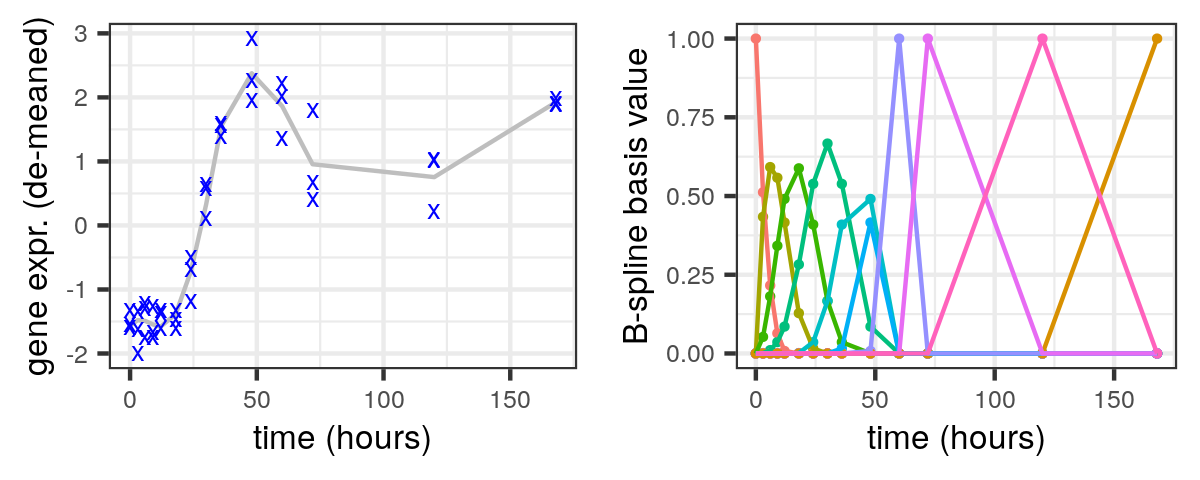
\includegraphics[width=0.980\linewidth,height=0.392\linewidth]{figure/example_genes-1} 

}

\caption[(Left) An example gene and its expression over time.
     (Right) The cubic B-spline with 7 degrees of freedom]{(Left) An example gene and its expression over time.
     (Right) The cubic B-spline with 7 degrees of freedom. }\label{fig:example_genes}
\end{figure}


\end{knitrout}
%


Let $\x_\n$ be the vector of observations 
$(\x_{\n 1}, ..., \x_{\n \ntimepoints})^T$.
Each cluster is characterized by a vector of regression coefficients 
$\beta_k$ and a variance $\tau^{-1}_k$; let $\theta_k = (\beta_k, \tau_k)$. 
The distribution of the data arising from cluster $k$ is 
\begin{align*}
p(\x_\n | \theta_k, \b_{n}) = 
\normdist{\x_\n | X\beta_k + \b_{n},
\tau^{-1}I_{\ntimepoints \times \ntimepoints}},
\end{align*}
where $\b_{n}$ is a gene-specific additive offset. 

The joint distribution equivalent to~\eqref{bnp_model}, 
except for the addition of a prior term for the additive offset: 
\begin{align*}
\MoveEqLeft
\logp(\x, \theta, \z, \nu) ={}
\nonumber\\&
    \sum_{n=1}^N \sum_{k=1}^{\kmax}
        \z_{\n\k} \left(
            \logp(\x_n \vert \theta_\k, \b_n) + \logp(\b_n) + \log \pi_\k
        \right) +
    \sum_{k=1}^{\kmax} \left(
        \log \pstick(\nuk) + \logp(\theta_\k) 
    \right).
\end{align*}
We use a normal prior for the shifts $\b_n$, 
a multivariate normal prior for the coefficients $\beta_n$,
and a gamma prior for the inverse variance $\tau$. 

Our variational distribution factorizes as~\eqref{vb_mf}, with the addition
of a factor for the additive shift that is conditional on $\z$: 
\begin{align*}
\q(\zeta \vert \eta) =
    \left( \prod_{\k=1}^{\kmax - 1} \q(\nuk \vert \eta) \right)
    \left( \prod_{\k=1}^{\kmax} \q(\theta_\k \vert \eta) \right)
    \left( \prod_{\n=1}^{\N} \q(\z_{\n} \vert \eta) 
    \q(\b_{\n} \vert \z_{\n}, \eta)\right).
\end{align*}
We set $\q(\b_{\n} \vert \z_{\n} = k, \eta)$ to be Gaussian, with mean and variance dependent on $k$. 
For simplicity in this application,
we let $\q(\theta_\k \vert \eta) = \delta (\theta \vert \eta)$, 
where $\delta(\cdot \vert \eta)$ denotes a point mass at a parameterized location. 

By parameterizing 
$\q(\z_{\n}, \b_{\n} \vert \eta) = \q(\z_{\n} \vert \eta)  \q(\b_{\n} \vert \z_{\n}, \eta)$ 
the optimal variational parameters for $\q(\z_{\n}, \b_{\n} \vert \eta)$ 
have a closed form given $\q(\nu, \theta \vert \eta)$. See TODO APPENDIX. 
Therefore, our model fits the global/local framework as discussed in TODO PREVIOUS SECTION,
with global latent variables $(\nu, \theta)$ and local latent variables $(\z, \b)$, and the size of the sensitivity matrix remains independent of $\ngenes$. 

We fit the initial model at $\alpha = 6$. 
\figref{gene_centroids} shows the inferred centroids 
$X\expect{}{\beta_k}$. 
\figref{gene_initial_coclustering} displays the inferred coclustering matrix. 
More precisely, let $\coclusteringmatr(\eta)$ denote the inferred coclustering matrix; 
its $i,j$-th entry is the
posterior probability that gene $i$ belongs to the same cluster
as gene $j$, given by 
\begin{align*}
\coclusteringmatr_{ij}(\eta) 
&= \expect{\q(\z\vert\eta)}{\ind{\z_{i} = \z_{j}}} \\
&= \sum_{k=1}^{\kmax}\left(\expect{\q(\z_i\vert\eta)}{\z_i = k}
\expect{\q(\z_j\vert\eta)}{\z_j = k}\right).
\end{align*}

Next, we evaluate the sensitivity of the inferred coclustering matrix to 
both parametric and functional perturbations to the stick distribution. 


\begin{knitrout}
\definecolor{shadecolor}{rgb}{0.969, 0.969, 0.969}\color{fgcolor}\begin{figure}[!h]

{\centering 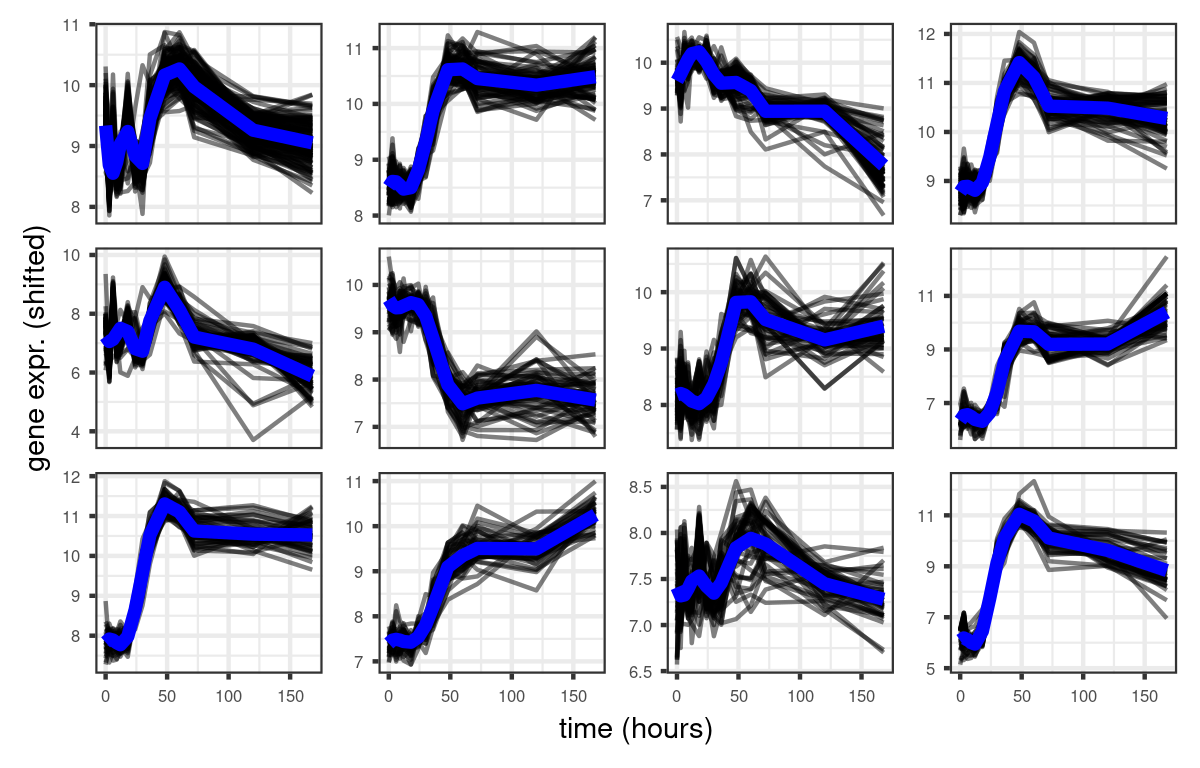
\includegraphics[width=0.980\linewidth,height=0.627\linewidth]{figure/gene_centroids-1} 

}

\caption[In blue, inferred centroids from the twelve most occupied clusters.
    In grey, gene expressions averaged over replicates and
    shifted by their inferred intercepts]{In blue, inferred centroids from the twelve most occupied clusters.
    In grey, gene expressions averaged over replicates and
    shifted by their inferred intercepts. }\label{fig:gene_centroids}
\end{figure}


\end{knitrout}



\begin{knitrout}
\definecolor{shadecolor}{rgb}{0.969, 0.969, 0.969}\color{fgcolor}\begin{figure}[!h]

{\centering 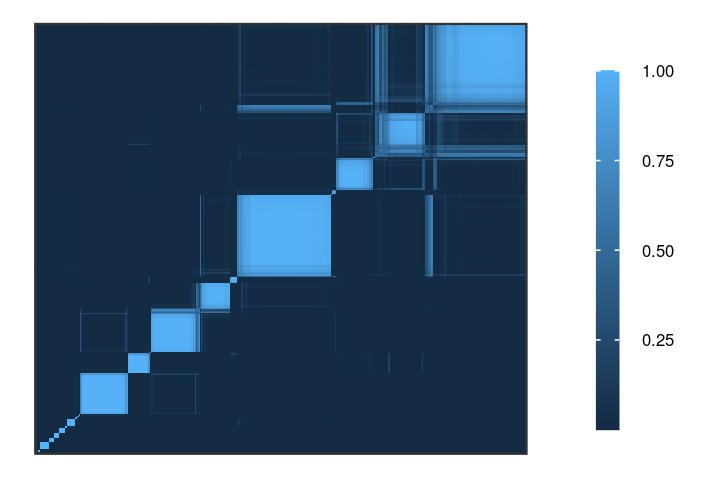
\includegraphics[width=0.588\linewidth,height=0.400\linewidth]{figure/gene_initial_coclustering-1} 

}

\caption[The inferred co-clustering of gene expressions at $\alpha = 3.$ ]{The inferred co-clustering of gene expressions at $\alpha = 3.$ }\label{fig:gene_initial_coclustering}
\end{figure}


\end{knitrout}


\subsubsection*{Sensitivity analysis}

We first evaluate the sensitivity of the coclustering matrix $\coclusteringmatr$ 
to the choice of the $\alpha$ parameter in the
$\betadist{\nuk \vert 1, \alpha}$ stick distribution. 
The initial coclustering matrix obtained at $\alpha = 6$ is shown in \figref{gene_initial_coclustering}. 
Let $\etaopt(\alpha)$ be the varaiational parameters refit at another $\alpha$,
and let $\etalin(\alpha)$ be variational parameters computed using the linear approximation with derivatives formed at $\alpha = 6$. 

Using the variational parameters at $\alpha = 6$ as an initialization, 
we refit the approximate posterior at $\alpha = 1$ and $\alpha = 11$. 
The effect of changing $\alpha$ on the co-clustering matrix is miniscule 
(\figref{gene_alpha_coclustering}). 
The largest absolute change in the entries of the matrices
$\coclusteringmatr(\etaopt(1)) - \coclusteringmatr(\etaopt(6))$ and 
$\coclusteringmatr(\etaopt(11)) - \coclusteringmatr(\etaopt(6))$ were
0.026 and 
0.015, respectively. 









\begin{knitrout}
\definecolor{shadecolor}{rgb}{0.969, 0.969, 0.969}\color{fgcolor}\begin{figure}[!h]

{\centering 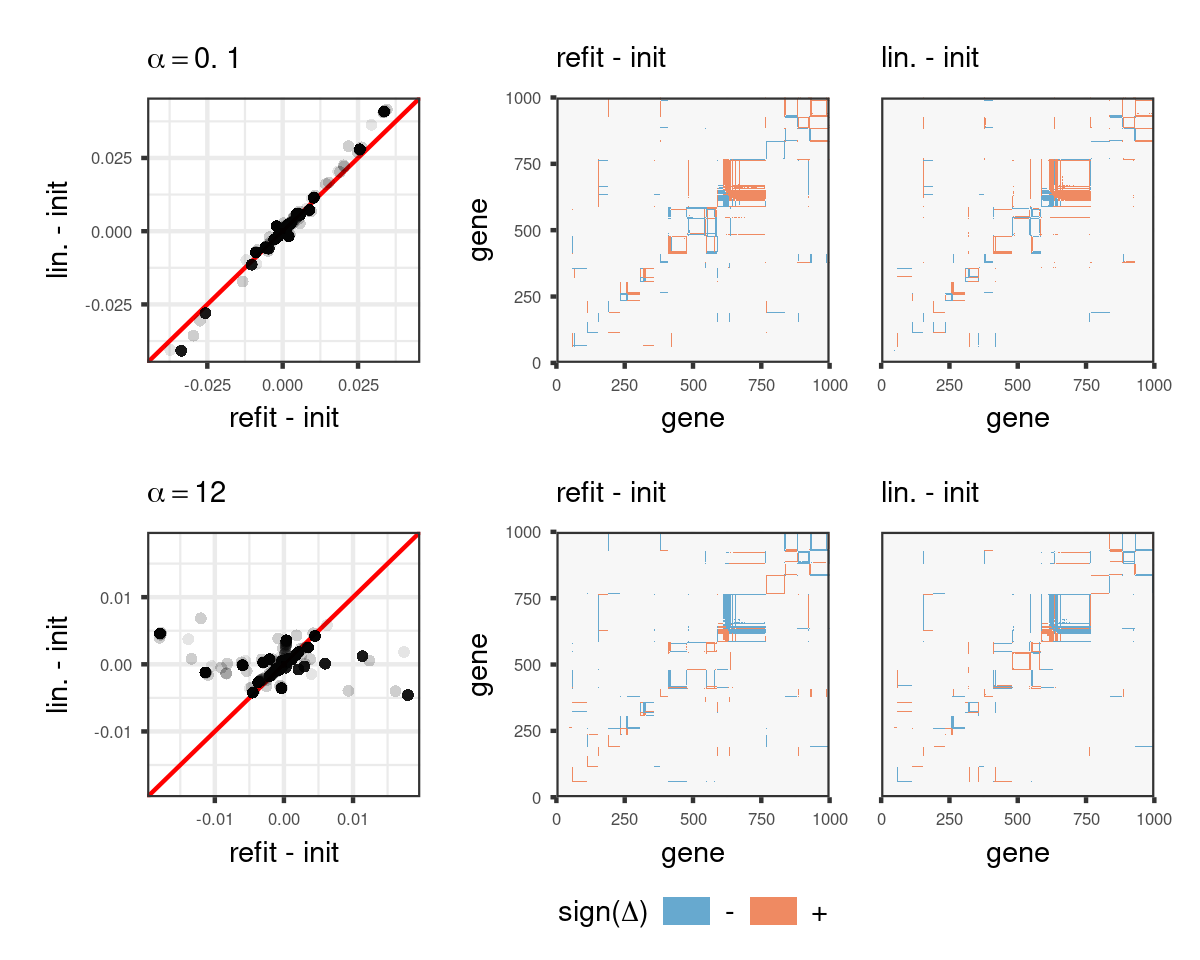
\includegraphics[width=0.980\linewidth,height=0.784\linewidth]{figure/gene_alpha_coclustering-1} 

}

\caption[Changes in the co-clustering matrix at alpha = 1 (top row)
     and alpha = 11 (bottom row),
     relative to the co-clustering matrix at alpha = 3.
     The left column plots differences predicted by the
     linear approximation against differences from a model refit.
     Each point represents an entry of the co-coclustering matrix.
     The middle and right columns display
     changes in the co-clustering matrix as obtained by the
     linear approximation and the model refit, respectively]{Changes in the co-clustering matrix at alpha = 1 (top row)
     and alpha = 11 (bottom row),
     relative to the co-clustering matrix at alpha = 3.
     The left column plots differences predicted by the
     linear approximation against differences from a model refit.
     Each point represents an entry of the co-coclustering matrix.
     The middle and right columns display
     changes in the co-clustering matrix as obtained by the
     linear approximation and the model refit, respectively.}\label{fig:gene_alpha_coclustering}
\end{figure}


\end{knitrout}





\begin{knitrout}
\definecolor{shadecolor}{rgb}{0.969, 0.969, 0.969}\color{fgcolor}\begin{figure}[!h]

{\centering 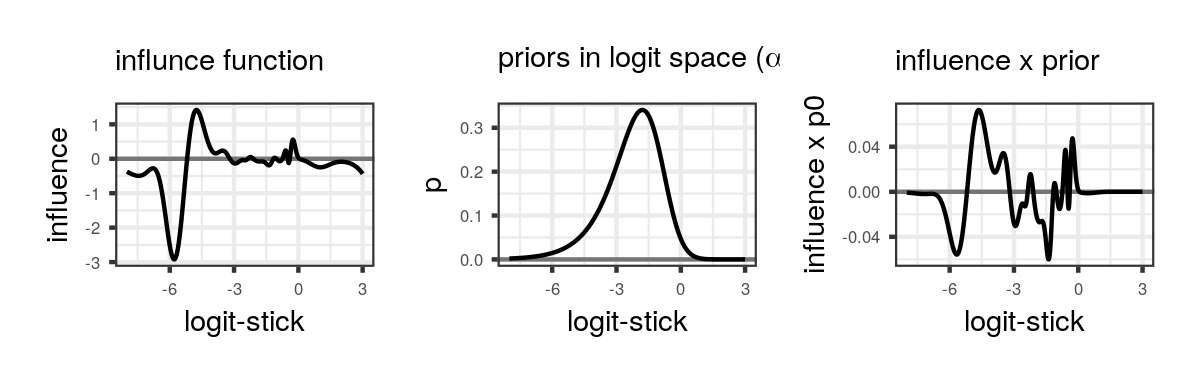
\includegraphics[width=0.980\linewidth,height=0.314\linewidth]{figure/gene_alpha_coclustering_influence-1} 

}

\caption[The influence function of $g_{ev}$, the sum of the eigenvalues of the coclustering Laplacian matrix]{The influence function of $g_{ev}$, the sum of the eigenvalues of the coclustering Laplacian matrix. }\label{fig:gene_alpha_coclustering_influence}
\end{figure}


\end{knitrout}





\begin{knitrout}
\definecolor{shadecolor}{rgb}{0.969, 0.969, 0.969}\color{fgcolor}\begin{figure}[!h]

{\centering 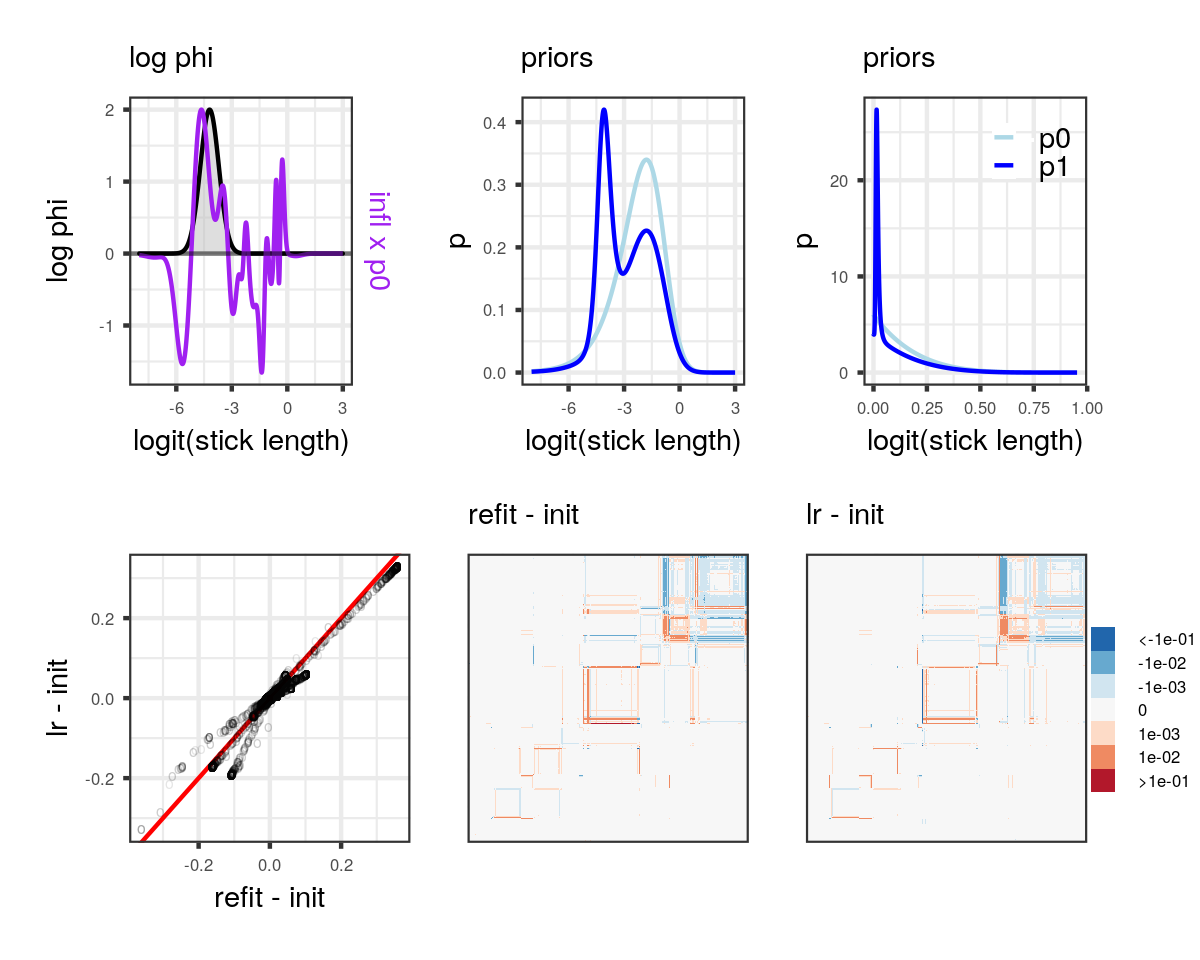
\includegraphics[width=0.980\linewidth,height=0.784\linewidth]{figure/gene_fpert_coclustering-1} 

}

\caption[Effect on the co-clustering matrix after a functional perturbation.
     log-phi (top left, in grey) is set to a Gaussian p.d.f]{Effect on the co-clustering matrix after a functional perturbation.
     log-phi (top left, in grey) is set to a Gaussian p.d.f. centered at mu = -4.2, and scaled to have L-infinity norm equal to two.
    The chosen log-phi roughly corresponds to a positive bump in the influence function of $g_{ev}$.}\label{fig:gene_fpert_coclustering}
\end{figure}


\end{knitrout}



\begin{knitrout}
\definecolor{shadecolor}{rgb}{0.969, 0.969, 0.969}\color{fgcolor}\begin{figure}[!h]

{\centering 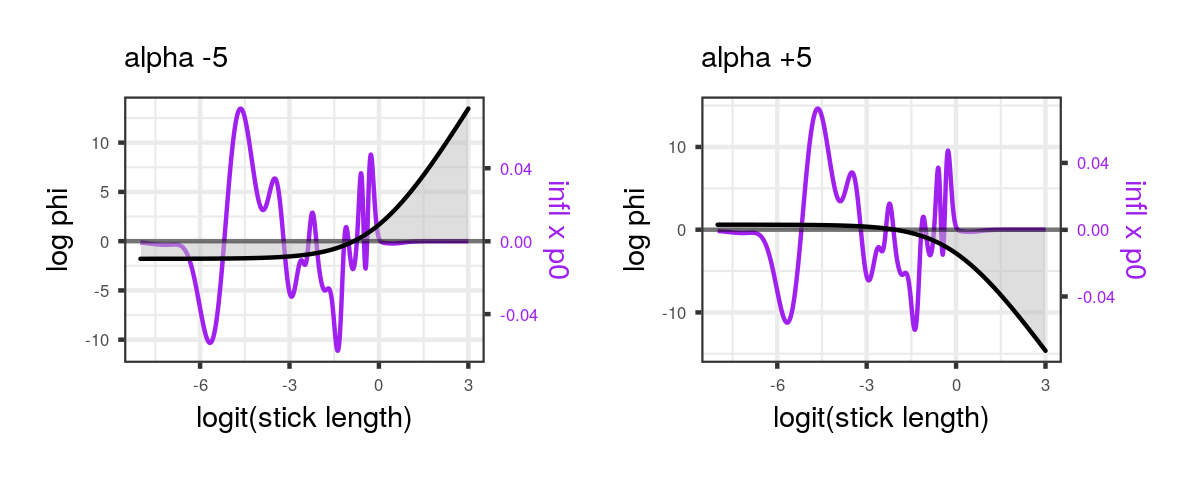
\includegraphics[width=0.980\linewidth,height=0.392\linewidth]{figure/alpha_pert_logphi-1} 

}

\caption[The log multiplicative perturbation $\log \phi$ corresponding to decreasing the $\alpha$ parameter by five (left) or increasing the $\alpha$ parameter by five (right)]{The log multiplicative perturbation $\log \phi$ corresponding to decreasing the $\alpha$ parameter by five (left) or increasing the $\alpha$ parameter by five (right). }\label{fig:alpha_pert_logphi}
\end{figure}


\end{knitrout}


\begin{table}[tb]
\centering
\caption{Compute time of results on the mice dataset. }
\begin{tabular}{|r|r|}
    \hline 
    & time (seconds) \\ 
    \hline 
    Initial fit & 25 \\
    \hline 
    Hessian solve for $\alpha$ sensitivity & 
        3.8\\
    Linear approx. $\eta^{lin}(\alpha)$ for $\alpha = 1$ & 
        0.0011\\
    Linear approx. $\eta^{lin}(\alpha)$ for $\alpha = 11$ & 
        0.0011\\
    Refit $\eta(\alpha)$ for $\alpha = 1$ & 
        16\\
    Refit $\eta(\alpha)$ for $\alpha = 11$ & 
        13\\
    \hline
    The influence function & 4.8\\ 
    Hessian solve for $\phi$ perturbation &
        3.2\\
    Linear approx. $\eta^{lin}(\epsilon)$ at $\epsilon = 1$ &
        0.00081\\
    Refit $\eta(\epsilon)$ at $\epsilon = 1$ &
        19\\
    \hline
\end{tabular}
\end{table}
